\documentclass{article}
\usepackage{graphicx}
\usepackage{float}
\usepackage[margin=.75in]{geometry}

\begin{document}

Code used in production of plots for this section can be found at https://github.com/cfmcginn/SystBio/tree/master/HW6.
\section{1.d}

\begin{figure}[H]
    \centering
    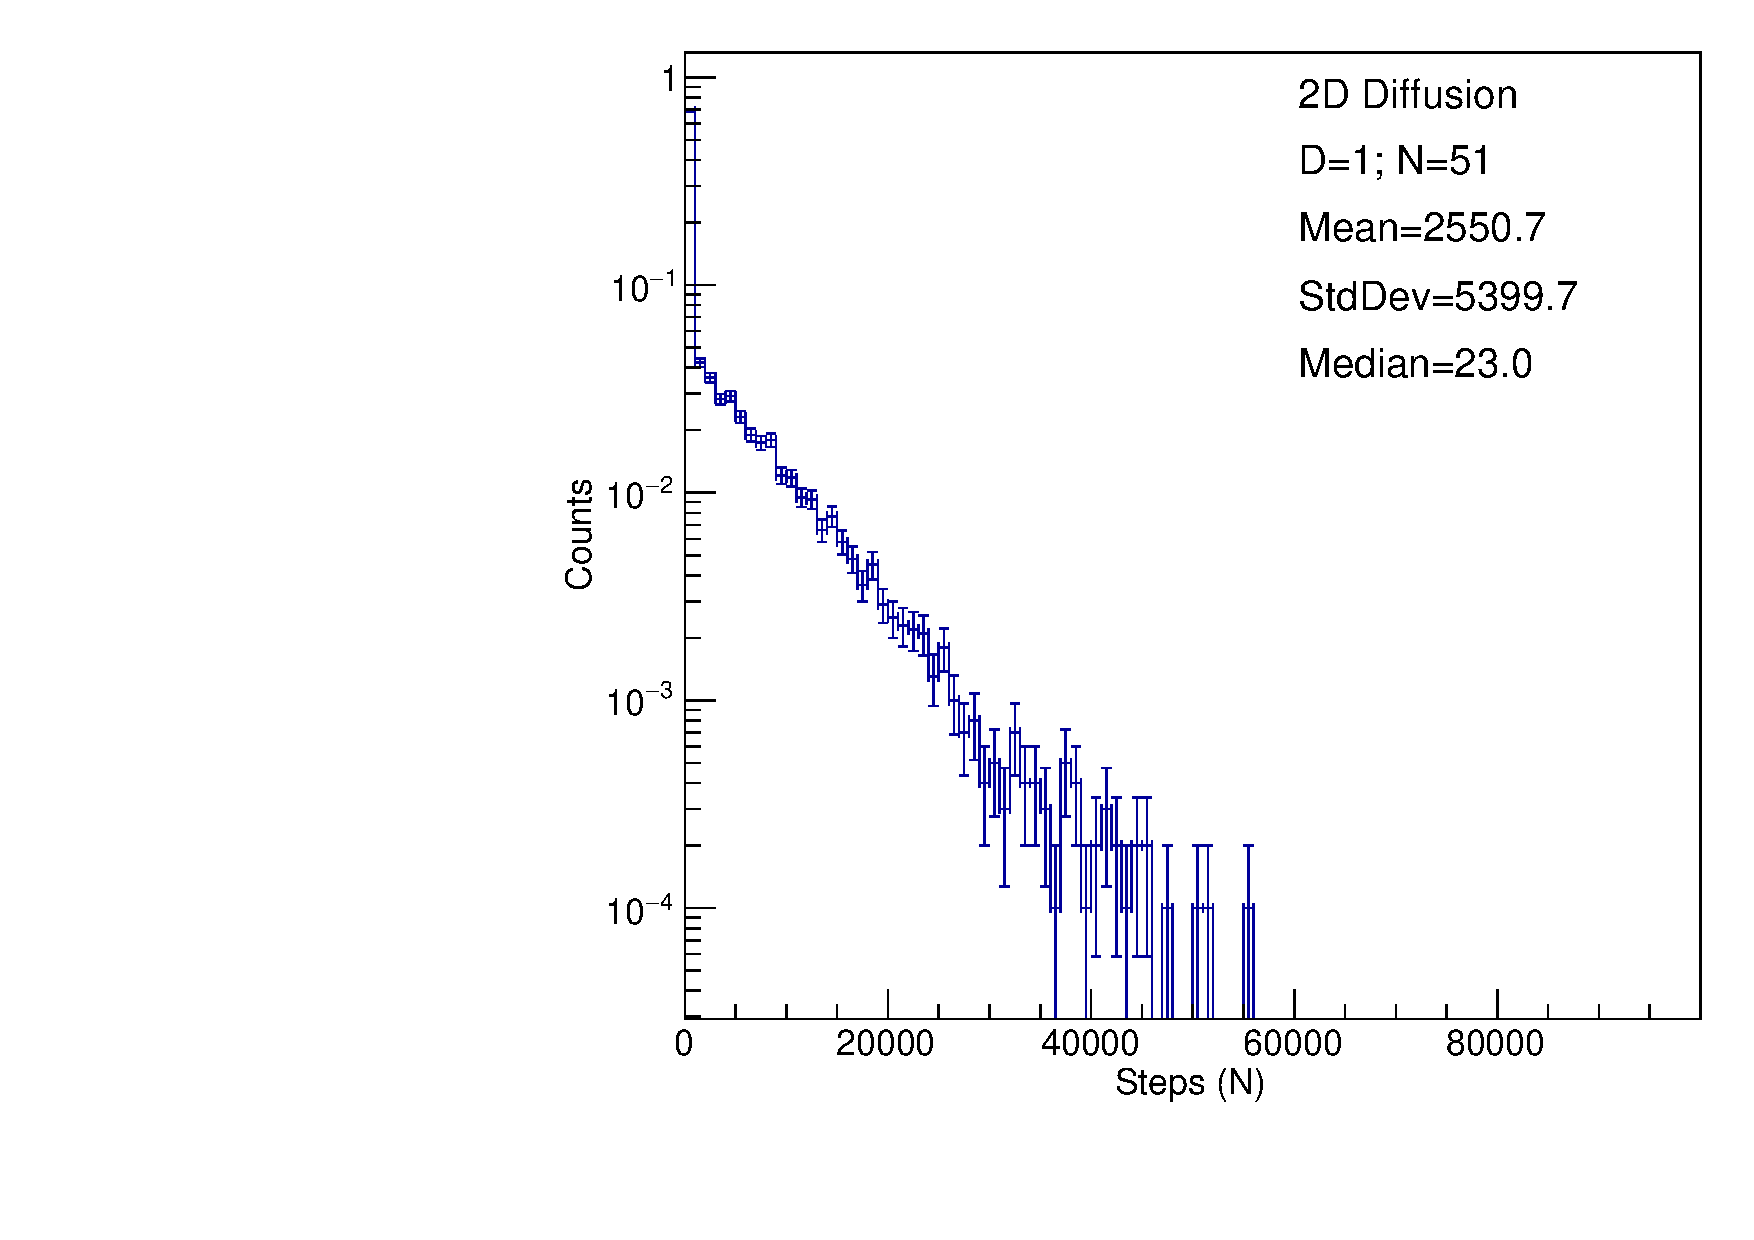
\includegraphics[width=.24\textwidth]{stepsToTarget_nSize51_D1.pdf} 
    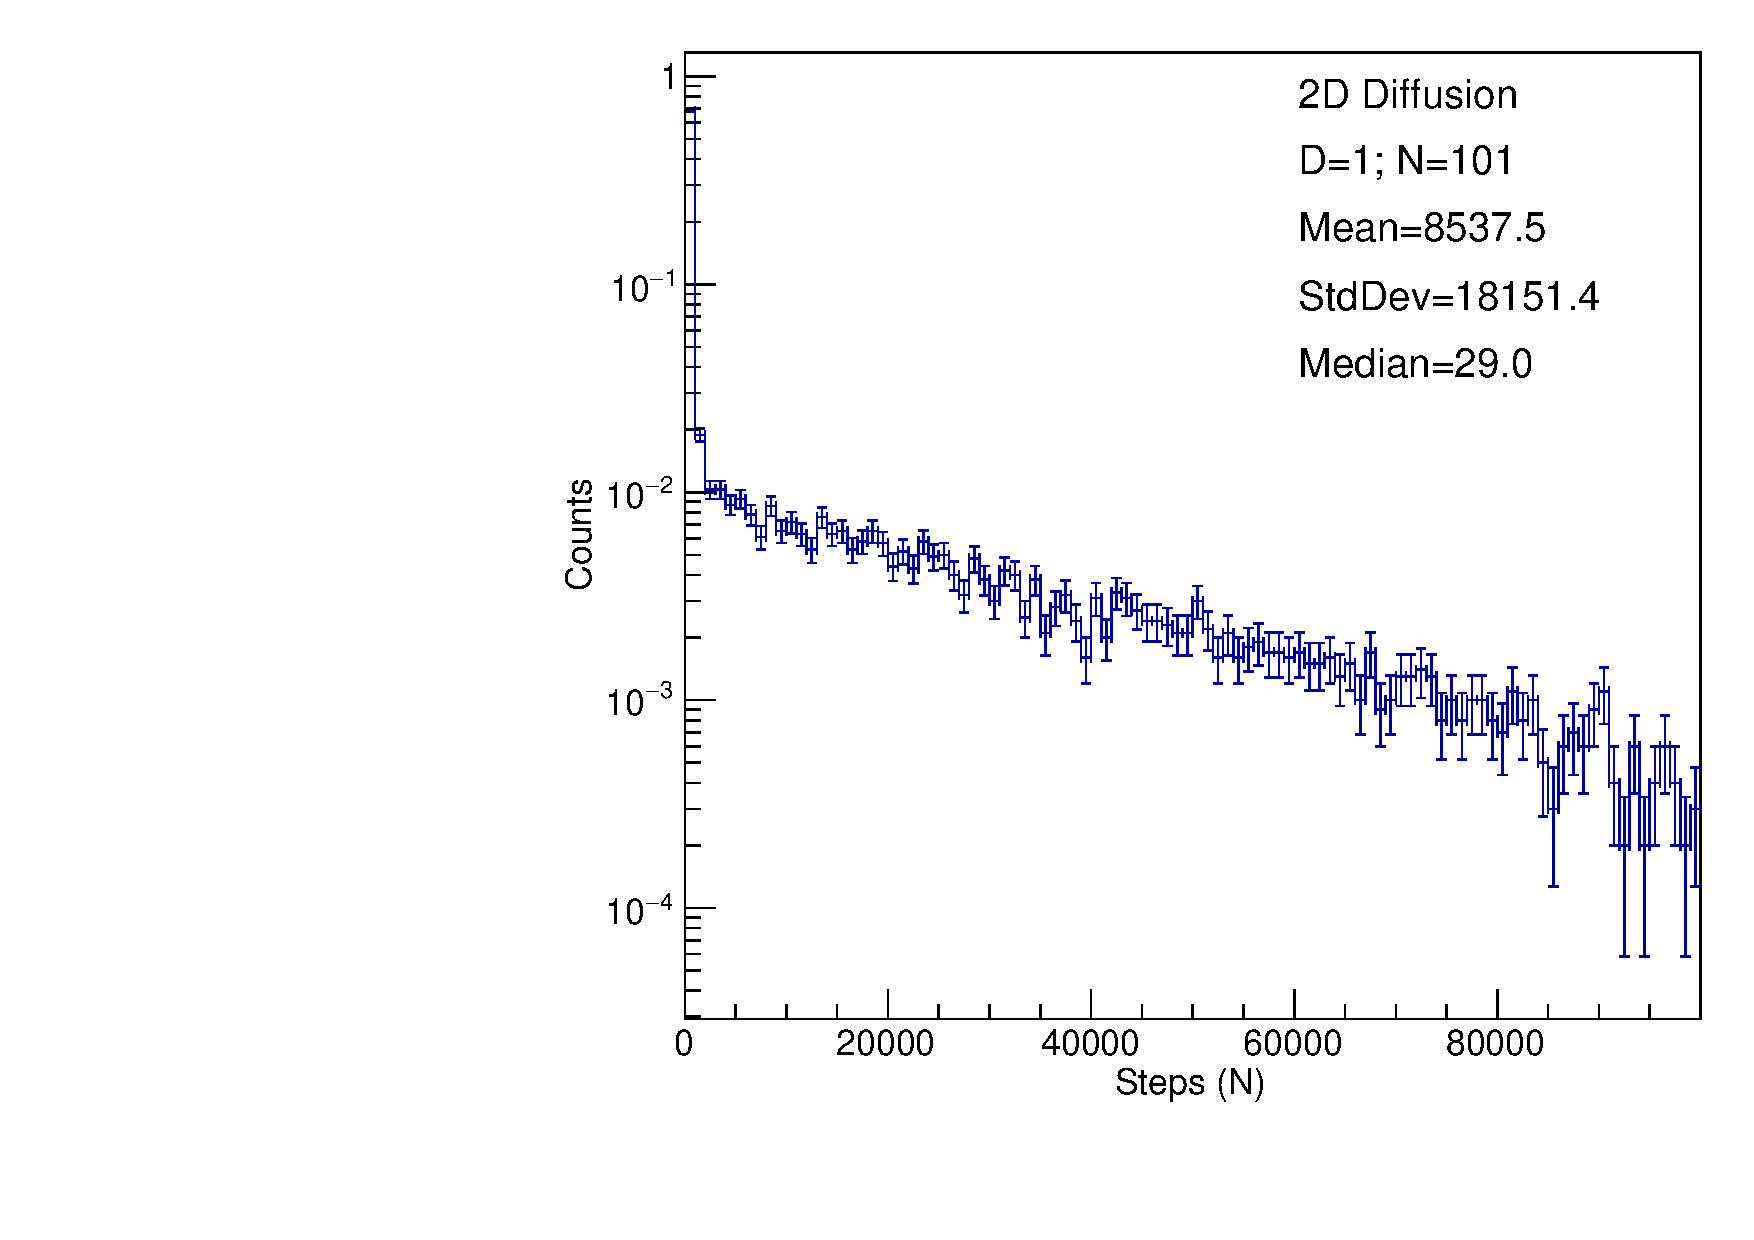
\includegraphics[width=.24\textwidth]{stepsToTarget_nSize101_D1.pdf} 
    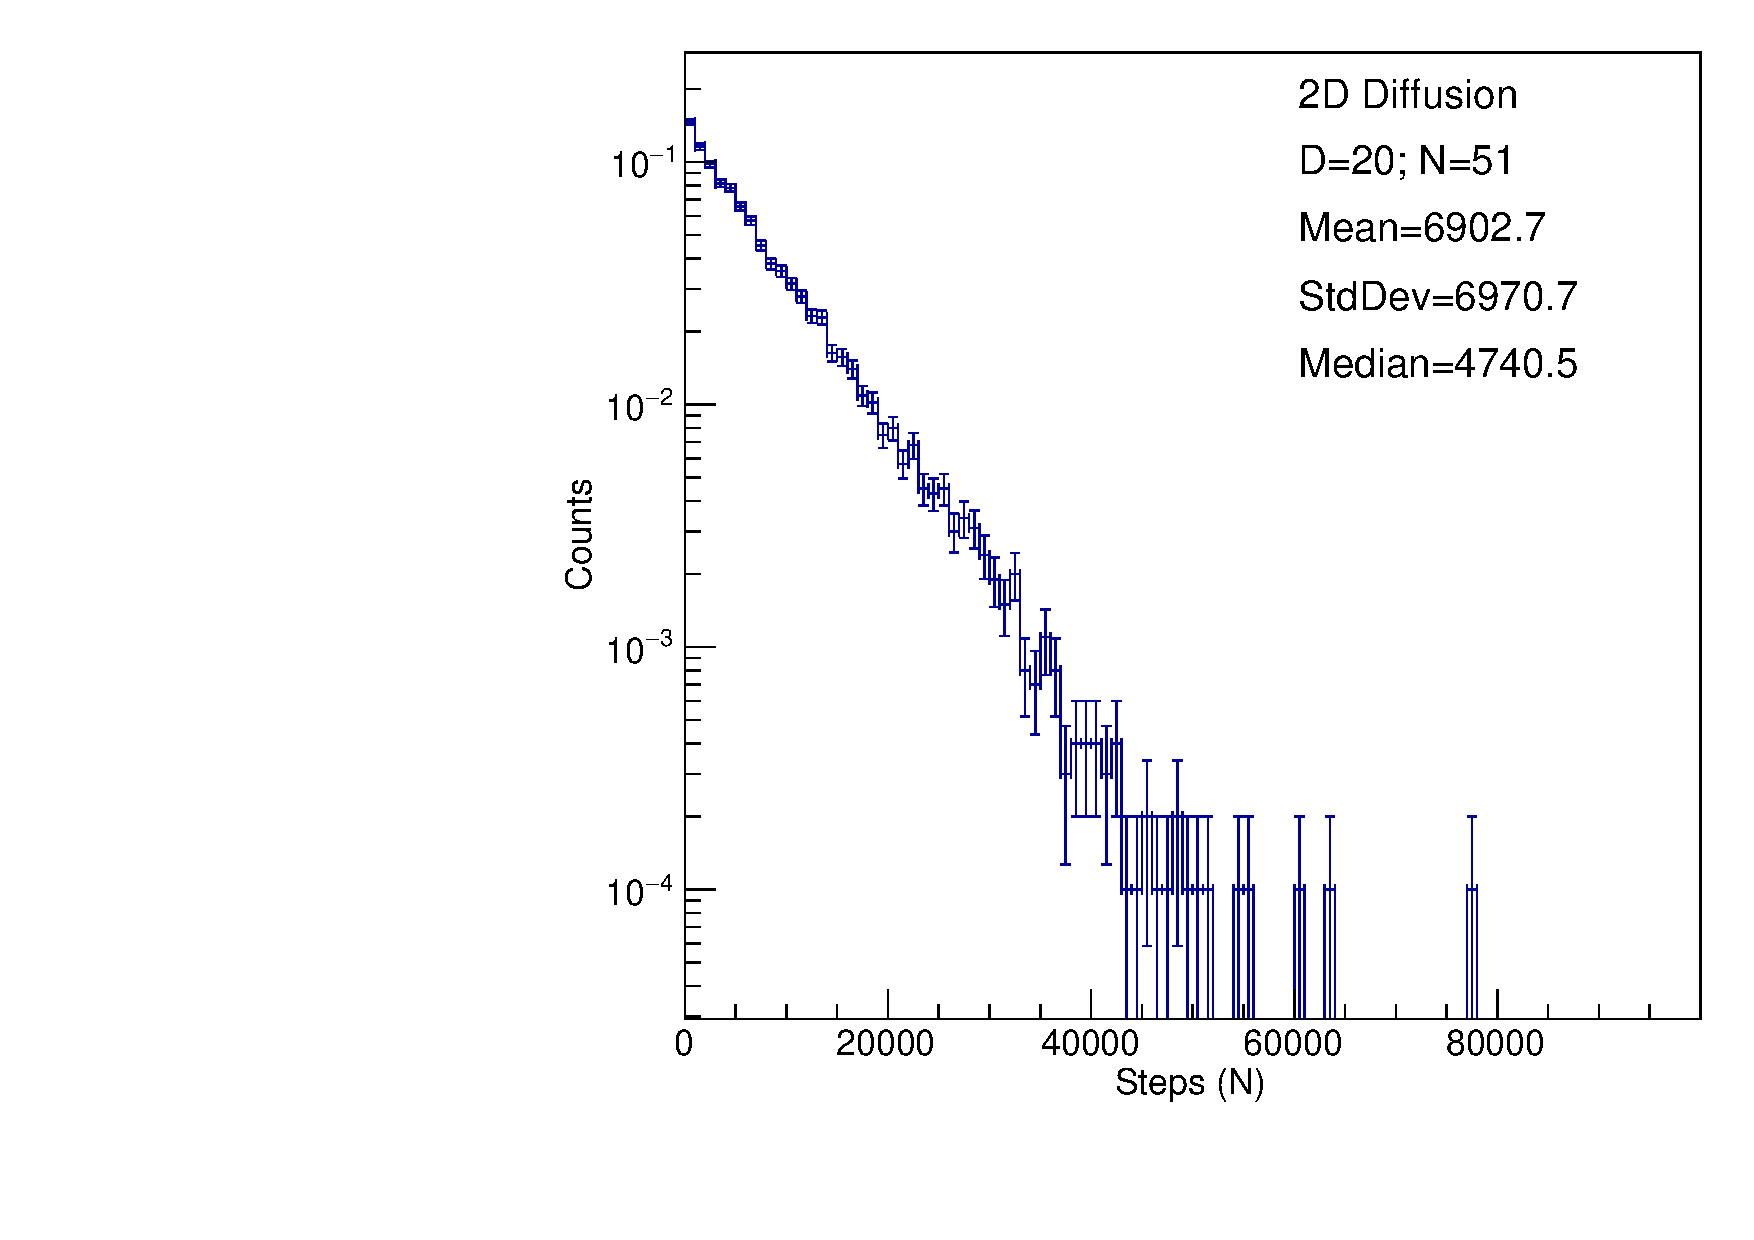
\includegraphics[width=.24\textwidth]{stepsToTarget_nSize51_D20.pdf} 
    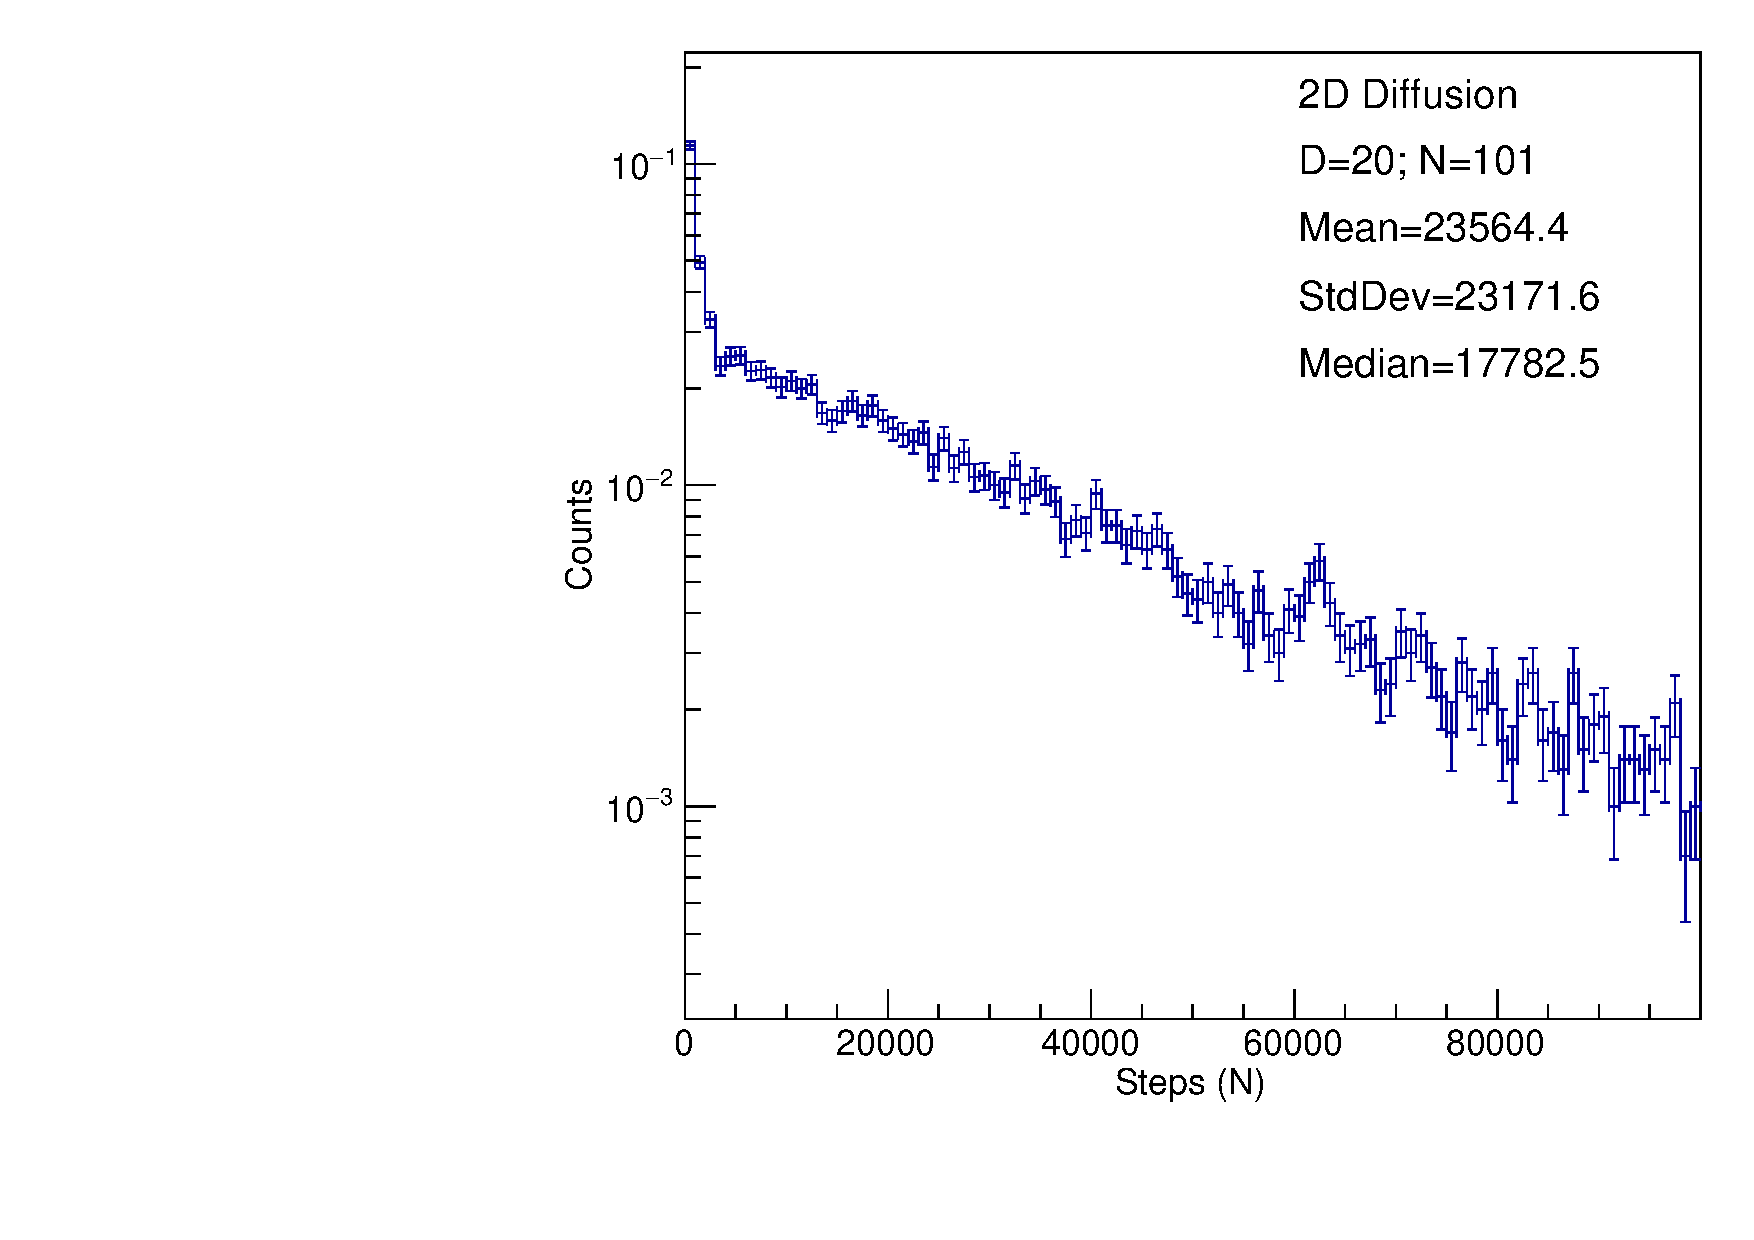
\includegraphics[width=.24\textwidth]{stepsToTarget_nSize101_D20.pdf} 
    \caption{Left to Right: (1) nGrid = 51, nTarget=1, (2) nGrid = 101, nTarget=1, (3) nGrid = 51, nTarget=20, (4) nGrid = 101, nTarget=20. All for pure 2-D diffusion}
    \label{fig1}
\end{figure}

Dependencies by taking ratios, mean goes as L*L*sqrt(d/2PI), standard deviation goes as L*L*sqrt(d/pi). So contra my guess, it is d$^{.5}$, not d, and there are constant factors accounting for the radial distance is distributed as 2pi in azimuthal angle.

\section{1.e}

\begin{figure}[H]
    \centering
    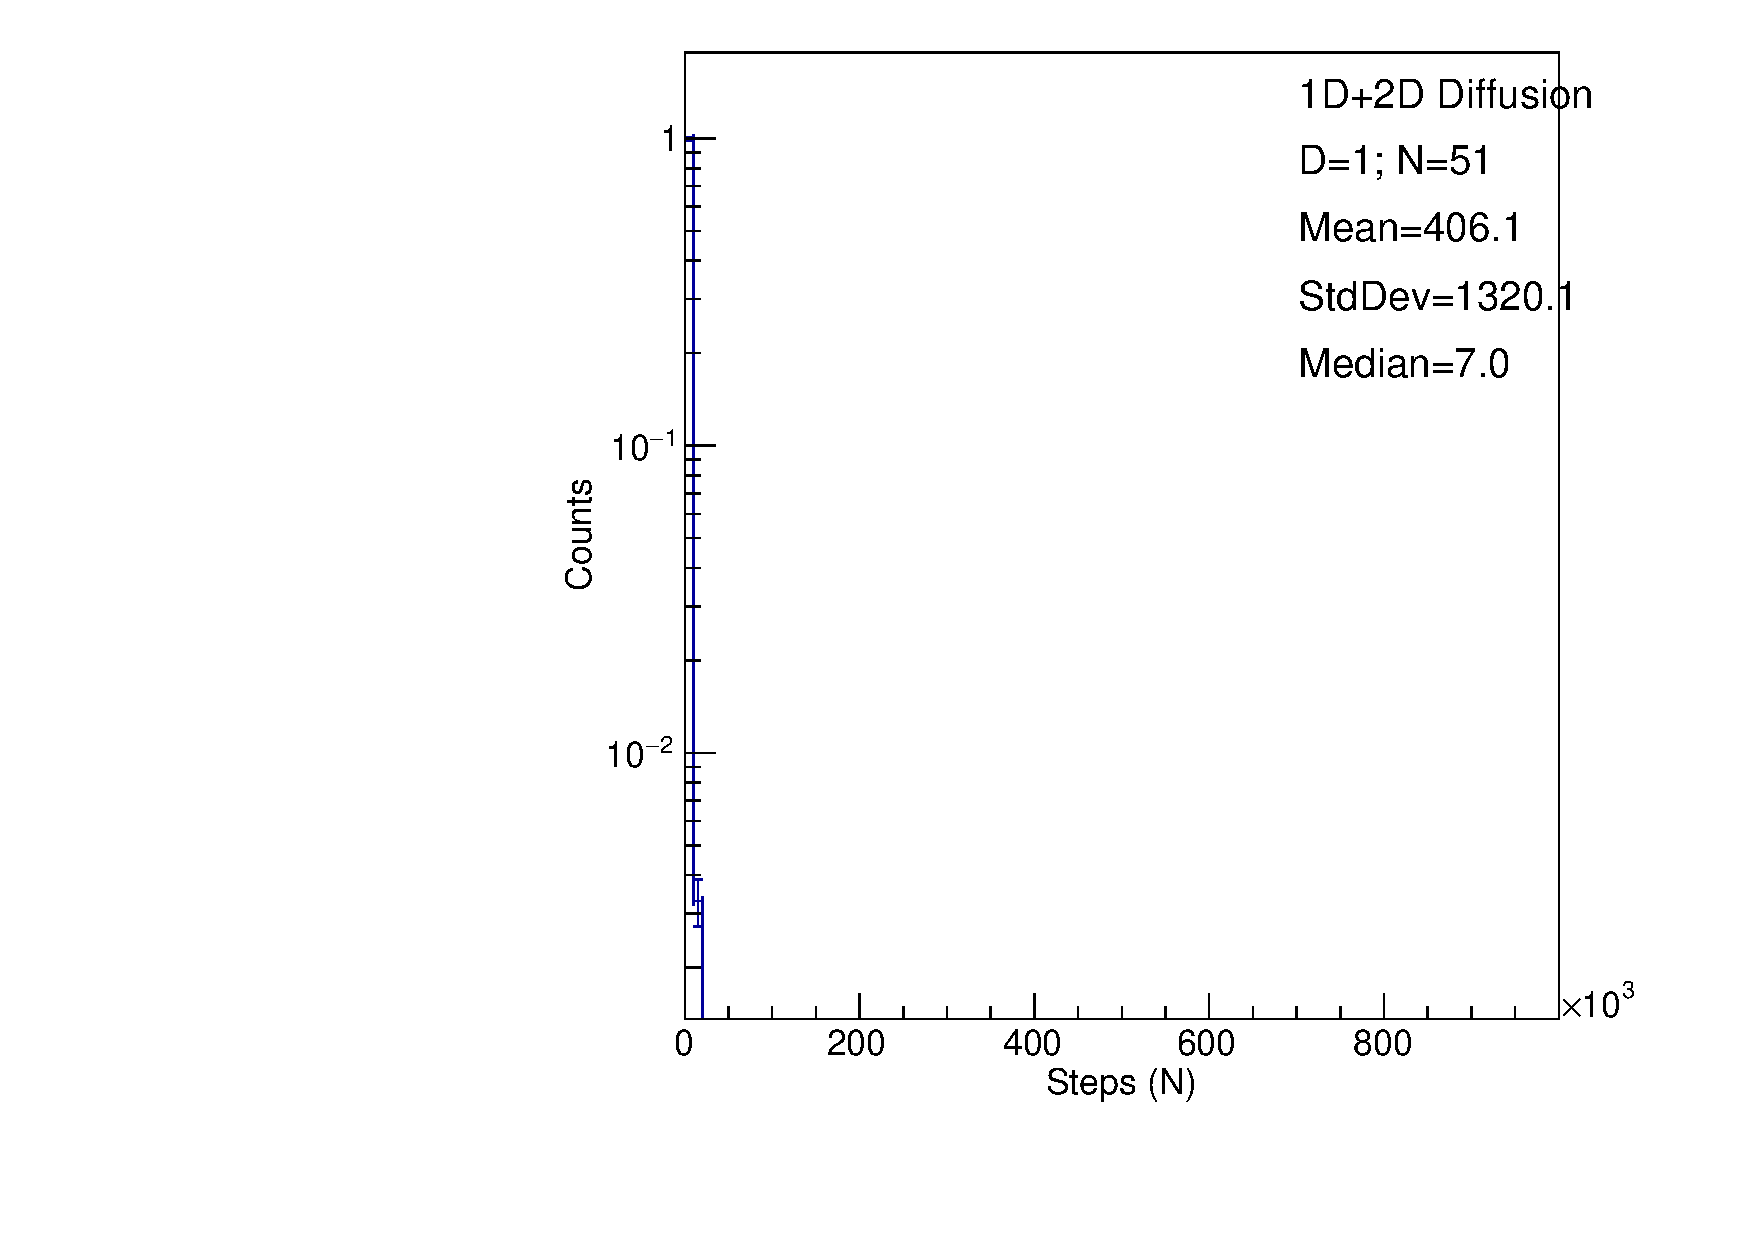
\includegraphics[width=.24\textwidth]{stepsToTargetAttach_nSize51_D1.pdf} 
    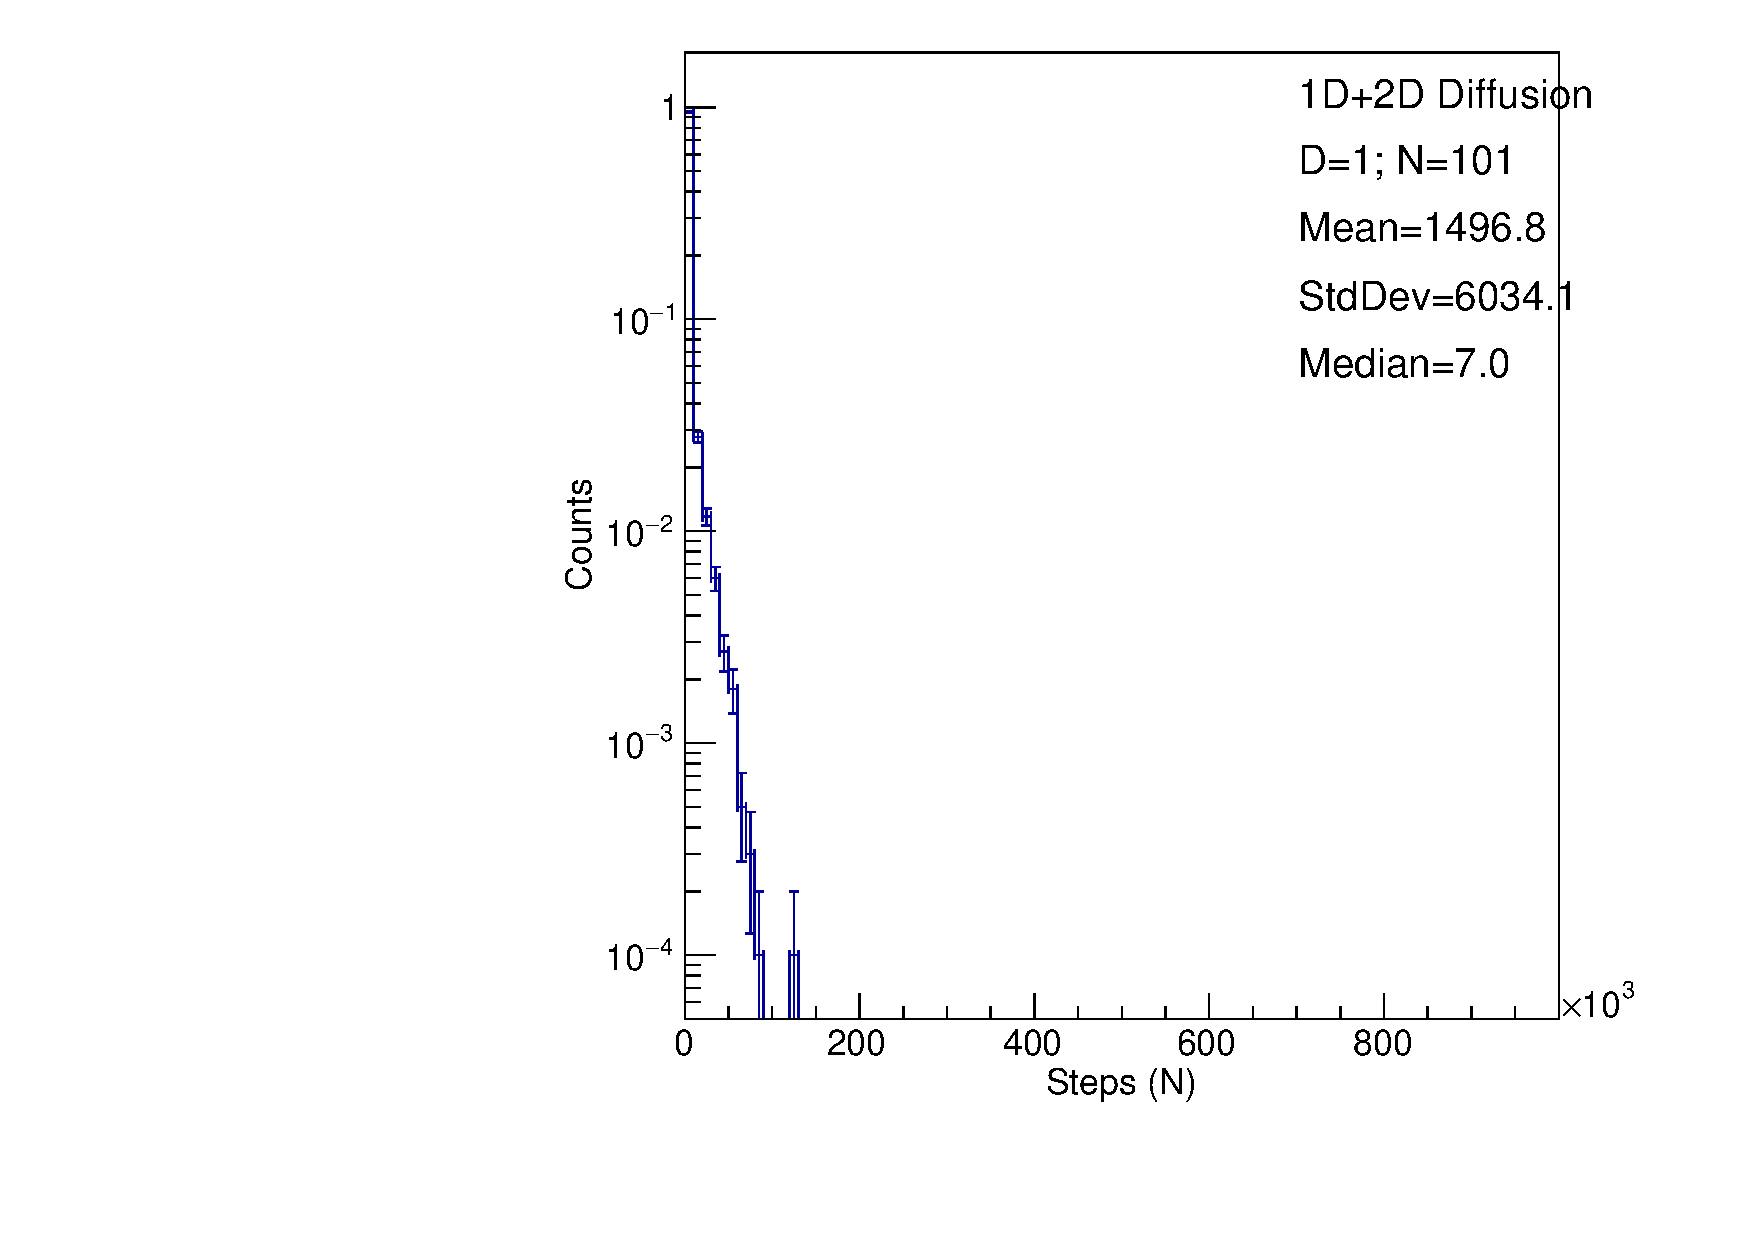
\includegraphics[width=.24\textwidth]{stepsToTargetAttach_nSize101_D1.pdf} 
    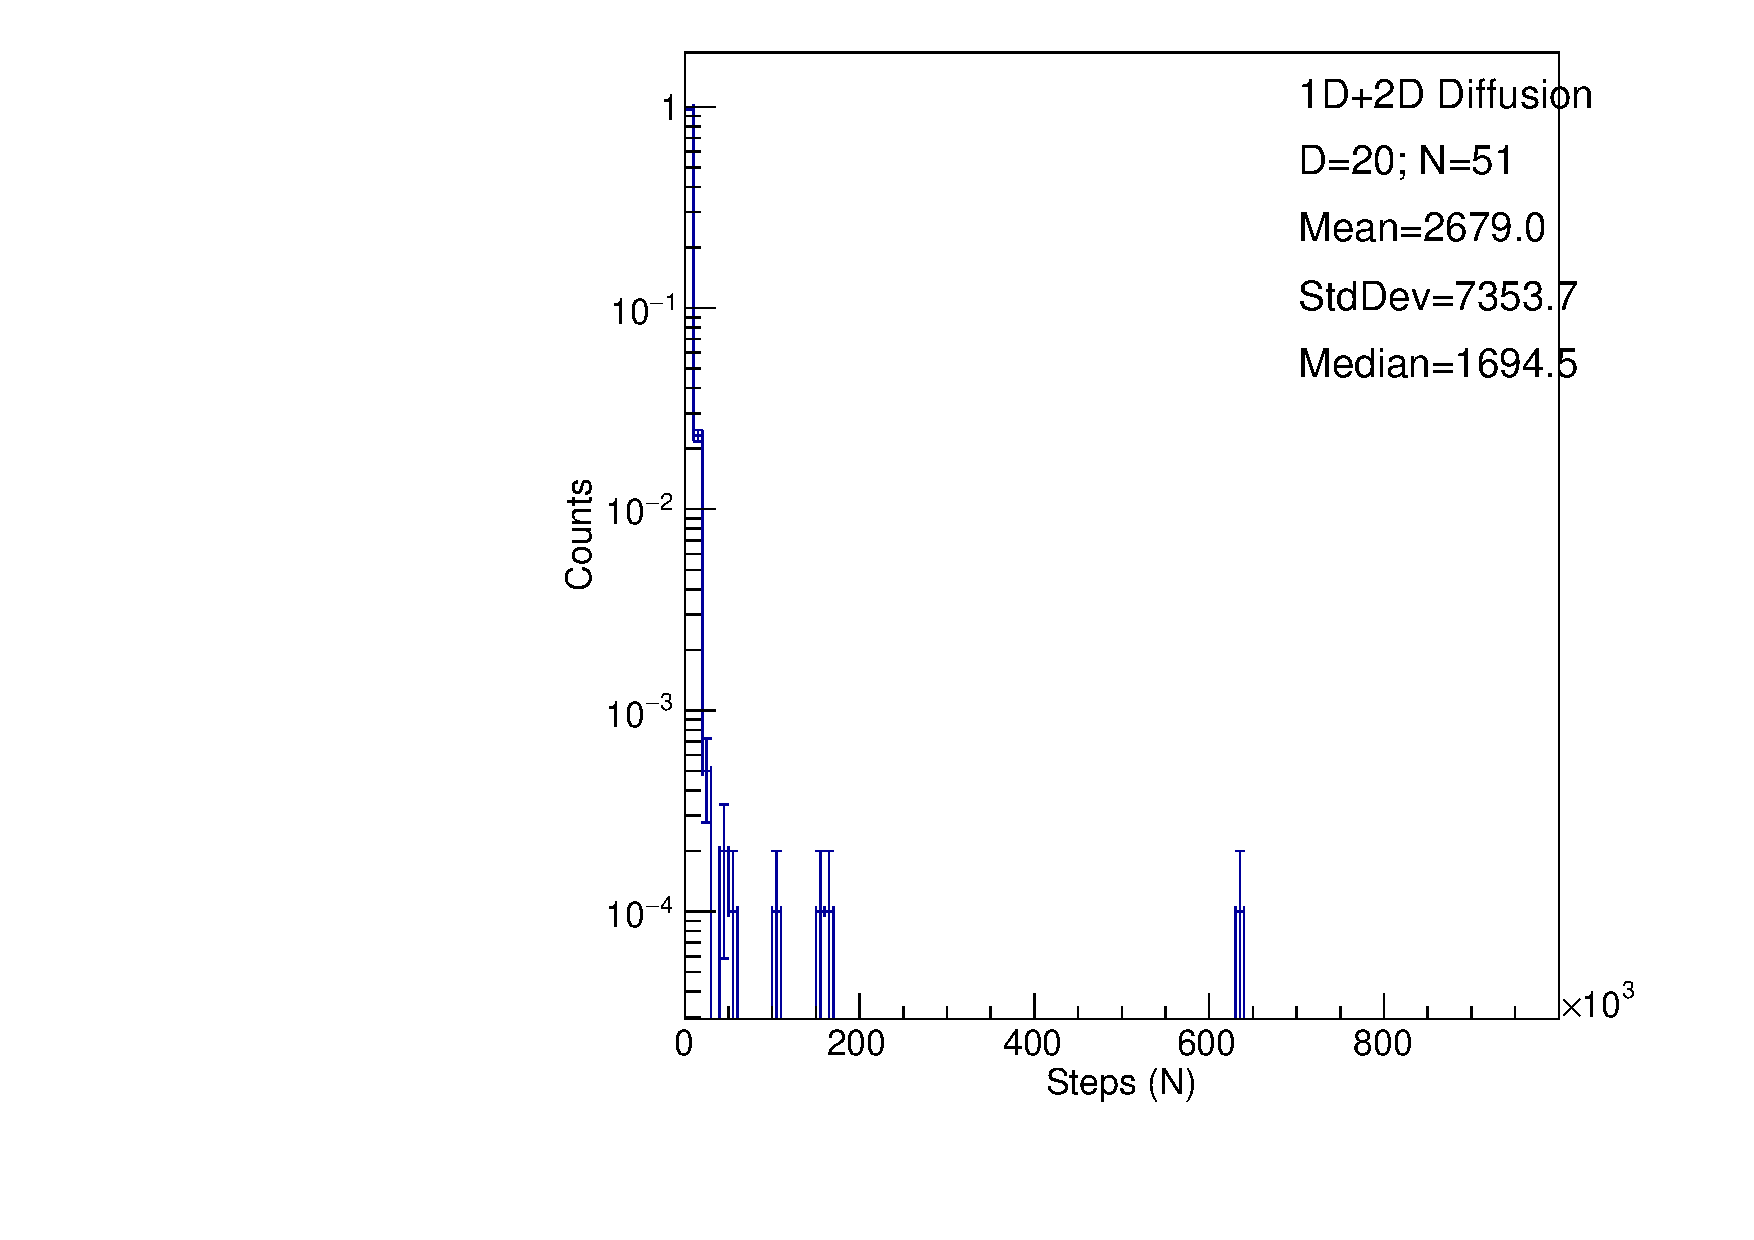
\includegraphics[width=.24\textwidth]{stepsToTargetAttach_nSize51_D20.pdf} 
    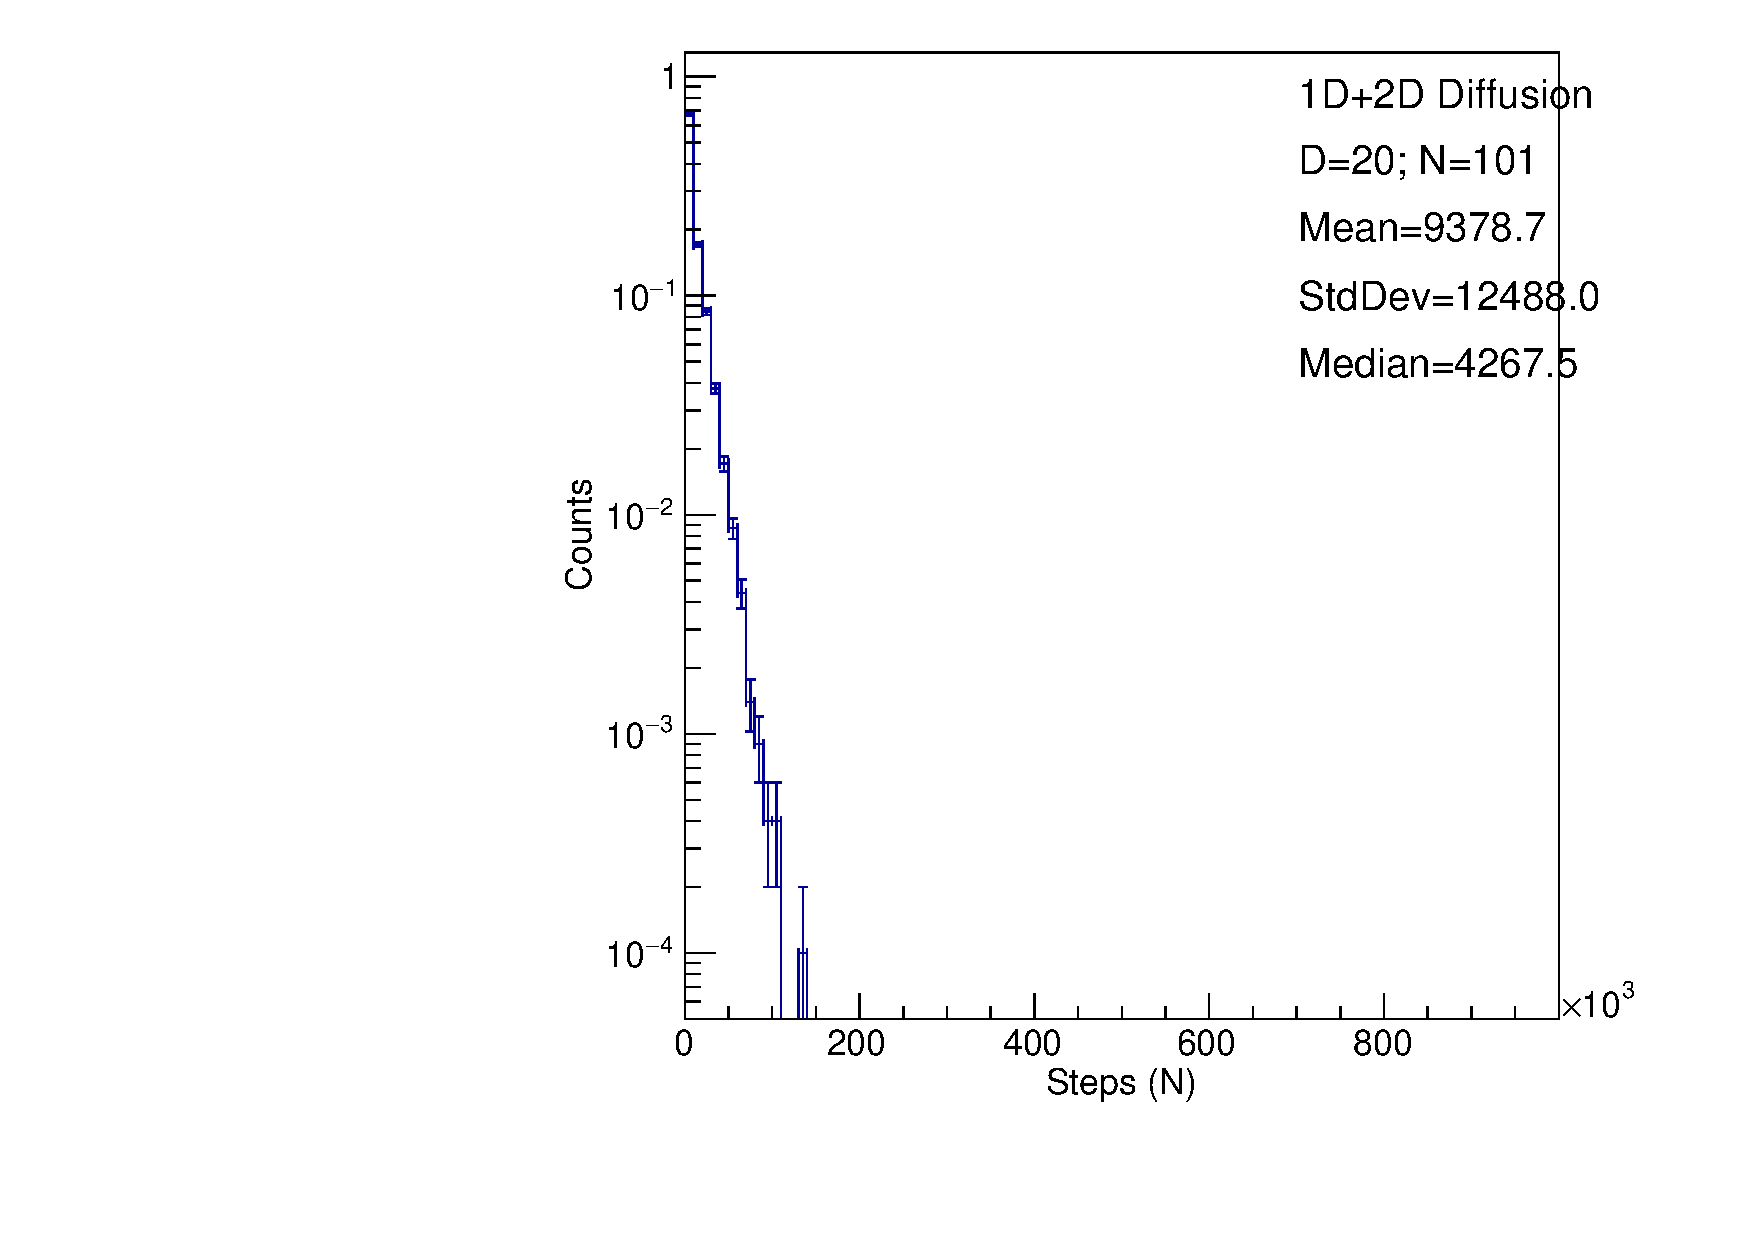
\includegraphics[width=.24\textwidth]{stepsToTargetAttach_nSize101_D20.pdf} 
    \caption{Left to Right: (1) nGrid = 51, nTarget=1, (2) nGrid = 101, nTarget=1, (3) nGrid = 51, nTarget=20, (4) nGrid = 101, nTarget=20. All for 2-D+1-D diffusion}
    \label{fig2}
\end{figure}

1-D diffusion reduces the total number of steps in all cases (mean, median, standard deviations), but not necessarily time. The latter depends on the average time to take each step in 2-D and 1-D cases.

\end{document}

